\section{Kết quả thực nghiệm}

Trong phần này, ta trình bày kết quả thực hiện các chức năng xử lý ảnh trên ảnh mẫu \texttt{Lena}, với kích thước \(512 \times 512\) pixels. Các chức năng xử lý ảnh bao gồm điều chỉnh độ sáng, độ tương phản, lật ảnh, chuyển đổi màu sắc, làm mờ/sắc nét ảnh, và cắt ảnh. Mỗi chức năng sẽ được trình bày kèm theo hình ảnh kết quả.

\begin{figure}[H]
	\centering
	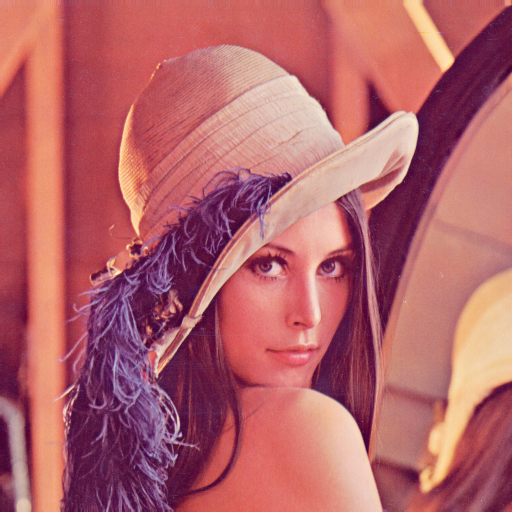
\includegraphics[width=0.5\textwidth]{imgs/lena.png}
	\caption{Ảnh mẫu Lena}
\end{figure}

\subsection{Điều chỉnh độ sáng}

\begin{figure}[H]
	\centering
	\subfloat[Tăng sáng (+40)]{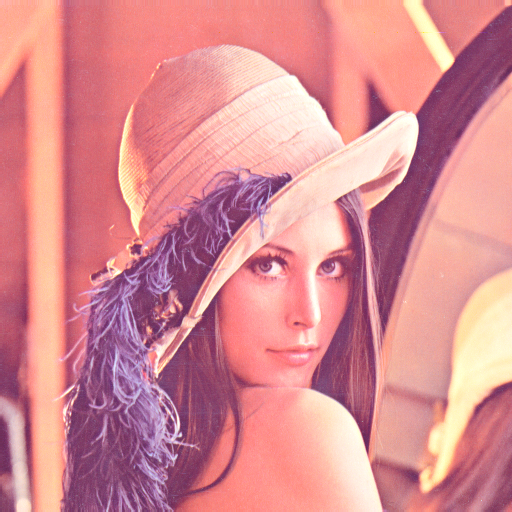
\includegraphics[width=0.45\textwidth]{imgs/lena_bright_up.png}}
	\hfill
	\subfloat[Giảm sáng (-40)]{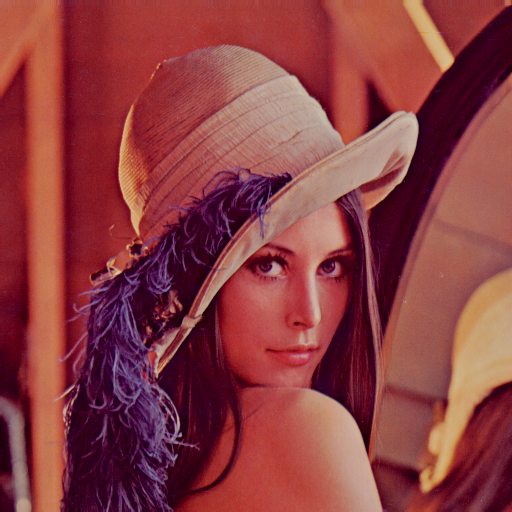
\includegraphics[width=0.45\textwidth]{imgs/lena_bright_down.png}}
	\caption{Ảnh sau khi điều chỉnh độ sáng}
\end{figure}

\subsection{Điều chỉnh độ tương phản}

\begin{figure}[H]
	\centering
	\subfloat[Tăng tương phản (1.5)]{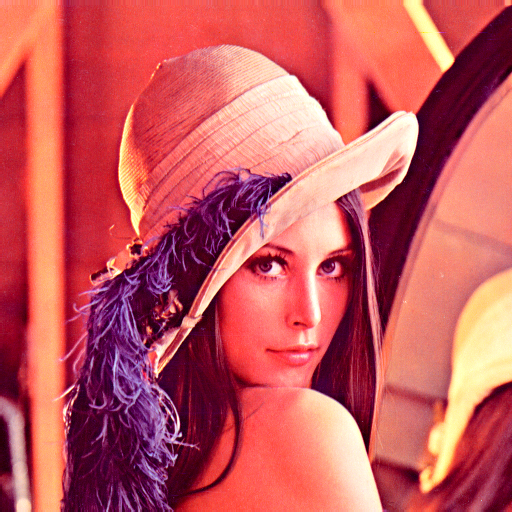
\includegraphics[width=0.45\textwidth]{imgs/lena_contrast_up.png}}
	\hfill
	\subfloat[Giảm tương phản (0.5)]{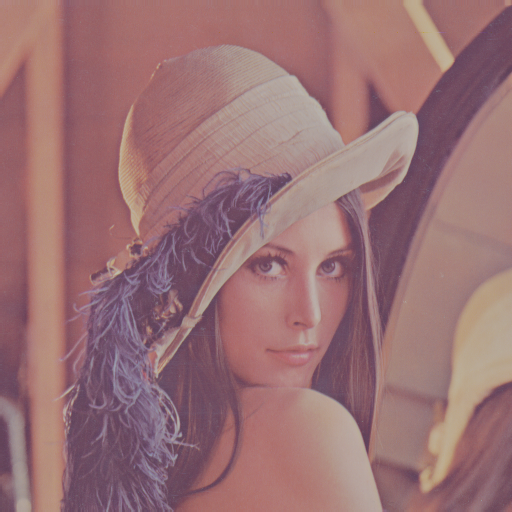
\includegraphics[width=0.45\textwidth]{imgs/lena_contrast_down.png}}
	\caption{Ảnh sau khi điều chỉnh độ tương phản}
\end{figure}

\subsection{Lật ảnh}

\begin{figure}[H]
	\centering
	\subfloat[Lật ngang]{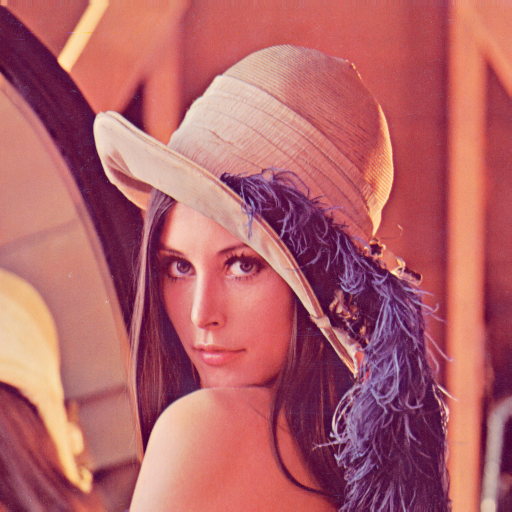
\includegraphics[width=0.45\textwidth]{imgs/lena_flip_horizontal.png}}
	\hfill
	\subfloat[Lật dọc]{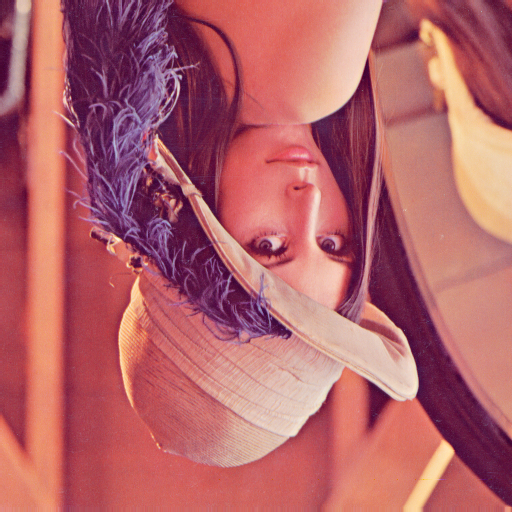
\includegraphics[width=0.45\textwidth]{imgs/lena_flip_vertical.png}}
	\caption{Kết quả lật ảnh}
\end{figure}

\subsection{Chuyển đổi màu sắc}

\begin{figure}[H]
	\centering
	\subfloat[Ảnh xám]{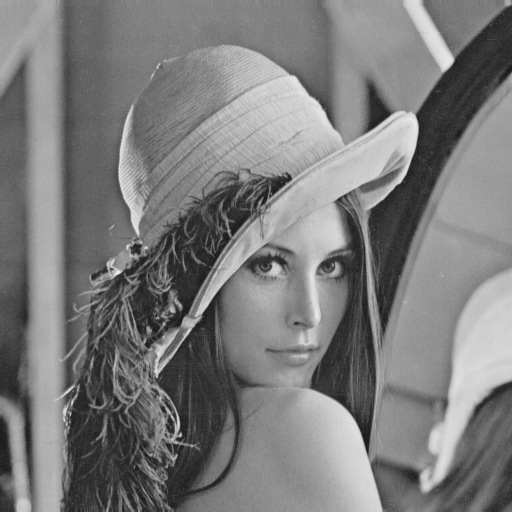
\includegraphics[width=0.45\textwidth]{imgs/lena_gray.png}}
	\hfill
	\subfloat[Ảnh sepia]{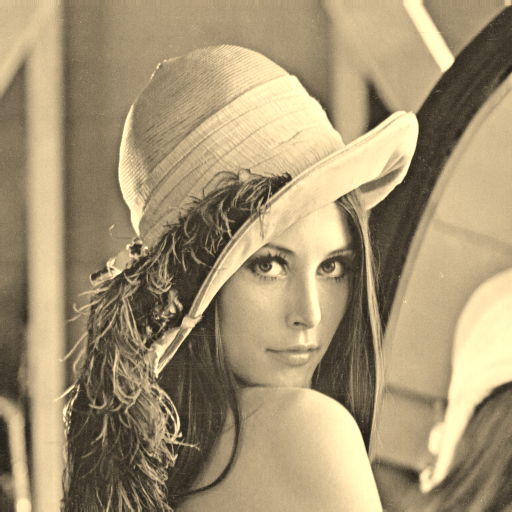
\includegraphics[width=0.45\textwidth]{imgs/lena_sepia.png}}
	\caption{Ảnh sau khi chuyển đổi màu sắc}
\end{figure}

\subsection{Làm mờ và sắc nét ảnh}

\begin{figure}[H]
	\centering
	\subfloat[Làm mờ (Blur)]{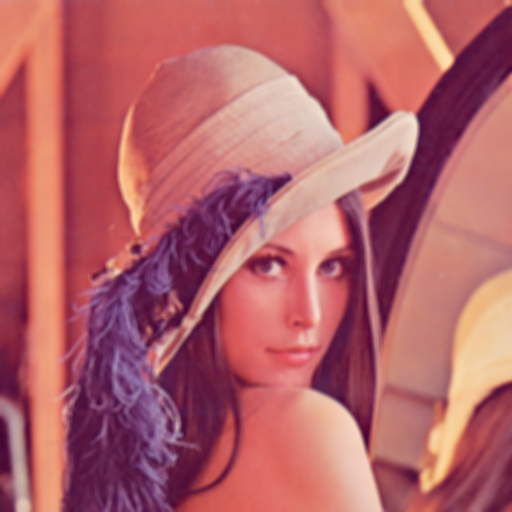
\includegraphics[width=0.45\textwidth]{imgs/lena_blur.png}}
	\hfill
	\subfloat[Làm sắc nét (Sharpen)]{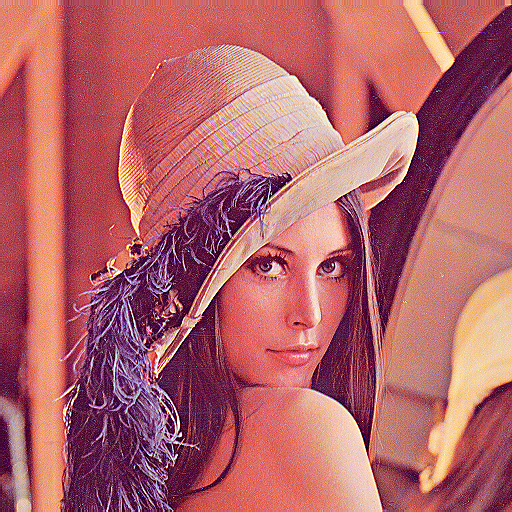
\includegraphics[width=0.45\textwidth]{imgs/lena_sharpen.png}}
	\caption{Ảnh sau khi áp dụng các bộ lọc}
\end{figure}

\subsection{Cắt ảnh theo khung hình vuông ở trung tâm}

\begin{figure}[H]
	\centering
	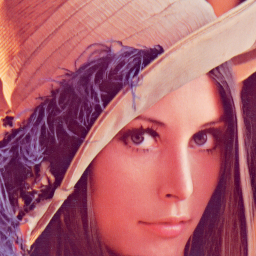
\includegraphics[width=0.5\textwidth]{imgs/lena_crop_center.png}
	\caption{Ảnh cắt ở trung tâm (size = \(256 \times 256\))}
\end{figure}

\subsection{Cắt ảnh theo khung hình tròn}

\begin{figure}[H]
	\centering
	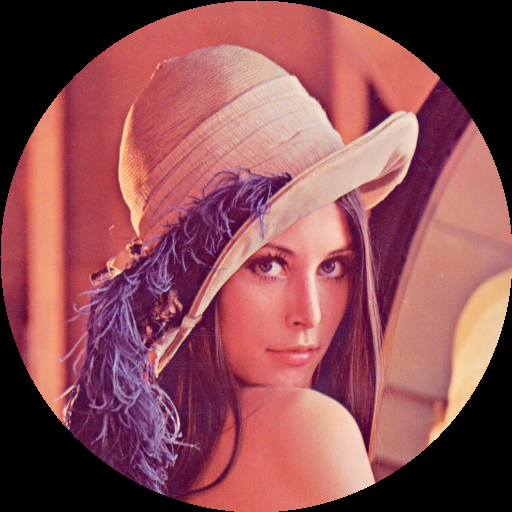
\includegraphics[width=0.5\textwidth]{imgs/lena_crop_circle.png}
	\caption{Ảnh cắt theo khung hình tròn}
\end{figure}

\subsection{Cắt ảnh theo khung hai hình ellipse chéo nhau}

\begin{figure}[H]
	\centering
	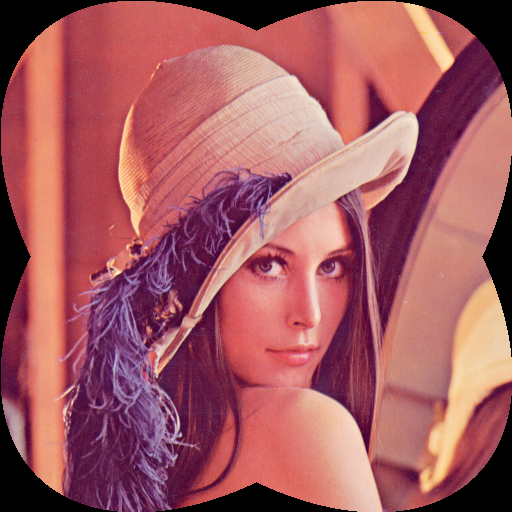
\includegraphics[width=0.5\textwidth]{imgs/lena_crop_ellipse.png}
	\caption{Ảnh cắt theo khung 2 hình ellipse chéo nhau (ratio = 0.6)}
\end{figure}

\subsection{Thời gian thực thi các chức năng}
\begin{table}[H]
	\centering
	\renewcommand{\arraystretch}{1.3}
	\caption{Thời gian thực thi của từng chức năng xử lý ảnh}
	\begin{tabular}{|p{10cm}|>{\raggedleft\arraybackslash}p{2cm}|}
		\hline
		\textbf{Chức năng}                            & \textbf{Thời gian} \\
		\hline
		Điều chỉnh độ sáng                            & 1.8ms              \\
		\hline
		Điều chỉnh tương phản                         & 4.4ms              \\
		\hline
		Lật ảnh ngang                                 & < 1ms              \\
		\hline
		Lật ảnh dọc                                   & < 1ms              \\
		\hline
		Chuyển ảnh RGB sang màu xám                   & 4.3ms              \\
		\hline
		Chuyển ảnh RGB sang màu sepia                 & 7.5ms              \\
		\hline
		Làm mờ ảnh                                    & 2760.7ms           \\
		\hline
		Làm sắc nét ảnh                               & 2635.1ms           \\
		\hline
		Cắt ảnh theo khung hình vuông ở trung tâm     & < 1ms              \\
		\hline
		Cắt ảnh theo khung hình tròn                  & 6.9ms              \\
		\hline
		Cắt ảnh theo khung hai hình ellipse chéo nhau & 15ms               \\
		\hline
	\end{tabular}
\end{table}

